\section{Introduction}

\begin{figure}[t]
    \centering
    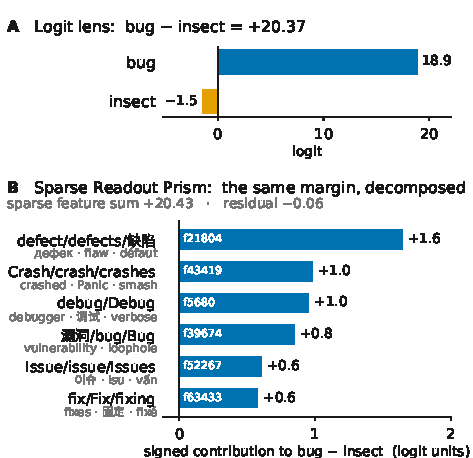
\includegraphics[width=\columnwidth]{figures/proto_token_lens/qwen2b_lens_prism_comparison_bug_insect/qwen2b_lens_prism_comparison_bug_insect.pdf}
    \caption{\textbf{A logit-lens margin and its decomposition into
    readout features.} \textbf{(A)} The logit lens scores the
    continuations \texttt{bug} and \texttt{insect} for Qwen3.5-2B on the
    prompt ``The programmer reproduced the crash and
    filed a'', giving a margin of \(+20.37\) in favor of \texttt{bug}.
    \textbf{(B)} SRP decomposes that same margin into signed
    readout-feature contributions, in logit units. The leading features
    all support \texttt{bug} and all concern software defects, with no
    insect-sense feature among them. Each bar is labeled with its
    feature id and that feature's three top-scoring LM-head rows, with
    lower-ranked rows in gray: the defect and bug
    features carry Chinese equivalents among their top rows, and the
    gray rows reach Russian, French, Korean, and Vietnamese;
    \Cref{sec:beyond-token} quantifies this cross-script structure.
    Small and token-form terms are hidden for readability; the sum and
    residual reported in the panel use the full decomposition.}
    \label{fig:main-lens-prism-comparison}
\end{figure}

Transformer language models score each vocabulary token by a dot product
between a final hidden state \(h\in\R^d\) and a row \(w_t\) of the
unembedding matrix \(\WU\in\R^{|\mathcal{V}|\times d}\)---the \emph{LM
head}, or \emph{readout}. Lens-style
methods~\citep{nostalgebraist2020,belrose2023tuned,pal2023future,ghandeharioun2024patchscopes}
reuse this map on intermediate hidden states and report what it yields:
vocabulary logits, token rankings, or distributions. The token, however,
is an ambiguous unit for that report: it is a surface unit of the
report, not of the readout,
and the mismatch runs both ways. Every sense of \texttt{bug}
shares one unembedding row, so the row's score conflates readings the
readout geometry keeps apart. Conversely, near-synonyms and
translation-equivalent tokens score through rows that share dominant
directions, so distinct tokens can stand in for one another as reports
of the same structure. Token identity is too coarse for the first
mismatch, too fine for the second. Lens methods supply much of the
evidence behind interpretability claims about intermediate computation:
which distinctions a hidden state carries, where in the stack a behavior
appears, how two models differ. Such claims are what auditing,
debugging, and targeted intervention are built on, and each is stated in
the unit the lens reports. A reported token that changes while the
structure it reads stays put is therefore not, by itself, evidence about
the computation.

Consider one hidden state from a software-context prompt: does the readout
favor the continuation \texttt{bug} over \texttt{insect}? The
logit lens reports the margin
(Figure~\ref{fig:main-lens-prism-comparison}, top) and stops there. Sparse
Readout Prism (SRP) asks how the margin is composed on the readout side:
which readout directions support it, which oppose it, and how much remains
unexplained (Figure~\ref{fig:main-lens-prism-comparison}, bottom). The
answer moves with the context: in an insect-context prompt the same
token's support reassembles around insect-sense readout directions
(\Cref{fig:selected-readout-prism-examples}). The converse ambiguity is
just as concrete: two Jacobian lenses \citep{gurnee2026workspace} that
differ only in their fitting corpora report different surface languages
on identical hidden states, while the decomposition shows the same
readout feature carrying both readings
(\S\ref{subsec:cross-lens}, \Cref{sec:beyond-token}). In both
directions, the shared feature account distinguishes a change in the
reported token from a change in the structure behind it.

SRP applies dictionary learning directly to LM-head rows: each row is
written as sparse coefficients over a shared overcomplete basis, plus a
residual. We call the shared directions \emph{readout
features}---features of LM-head rows rather than of hidden-state
activations. Selecting a token or contrast fixes a dense dot product
\(h^\top q\), where \(q\) is an LM-head row or row combination; we call
any such fixed combination a \emph{readout score}, and a \emph{contrast}
is the zero-sum case comparing alternatives, such as the logit
difference \(h^\top(w_A-w_B)\). Once a readout score is fixed, the
row-side coefficients combine with hidden-state projections
\(p_i(h)=h^\top d_i\) to give signed per-feature contributions in
original logit units, plus an explicit residual---readout features,
rather than tokens, are the unit in which SRP reads the score. TopK
dictionary fitting is a standard
primitive~\citep{makhzani2013ksparse,gao2024scaling}; the contribution
is the factorized readout and the selected-score interface it induces.

Nearby accounts differ in what they decompose. Activation SAEs decompose
the hidden state itself, learning corpus- and layer-specific bases for
\(h\)~\citep{bricken2023monosemanticity,cunningham2023sparse,gao2024scaling};
the SRP basis instead comes from the weights alone and exists before any
prompt. Residual-stream attribution decomposes how components wrote the
hidden state, SRP which directions a selected score reads from it---the
two are complementary. Direct LM-head geometry works on the same rows
SRP factorizes, but is not held to reproducing any particular score;
SRP is judged by whether it does, with an explicit error for each.

This paper makes three contributions, each supplying one property the
alternative unit needs:
\begin{itemize}
    \item \emph{A compositional readout-feature interface.} A weight-only
    sparse factorization of the LM head that turns any selected token
    logit, logit difference, or fixed vocabulary-row combination into
    readout-feature contributions plus an explicit residual in
    logit units, without prompt-, task-, or layer-specific
    training (\Cref{sec:method}).
    \item \emph{Distinct, reproducible, causally predictive structure.}
    On the six of eight models whose factorized head passes a
    replacement check on held-out states, SRP reconstructs selected
    scores more reliably than methods built directly on LM-head row
    geometry, and recovers token groupings those methods miss. Its
    explanations reproduce across independent training runs, and its
    feature contributions predict the measured effect of deleting
    individual features from the readout (\Cref{sec:results}).
    \item \emph{A cross-lens finding: corpus conditionality.}
    English- and Chinese-fitted Jacobian lenses report different
    surface languages on identical hidden states while the same SRP
    feature stays dominant on 77 of 80 prompts: the reported language
    follows the lens's fitting corpus, not a change in the structure
    being read (\Cref{sec:beyond-token}).
\end{itemize}
